
% This LaTeX was auto-generated from MATLAB code.
% To make changes, update the MATLAB code and republish this document.

\documentclass{article}
\usepackage{graphicx}
\usepackage{color}

\sloppy
\definecolor{lightgray}{gray}{0.5}
\setlength{\parindent}{0pt}

\begin{document}

    
    
\section*{MATLAB programming course for beginners, supported by Wagatsuma Lab@Kyutech}

\begin{par}
/* The MIT License (MIT): Copyright (c) 2022 Hiroaki Wagatsuma and Wagatsuma Lab@Kyutech
\end{par} \vspace{1em}
\begin{par}
Permission is hereby granted, free of charge, to any person obtaining a copy of this software and associated documentation files (the "Software"), to deal in the Software without restriction, including without limitation the rights to use, copy, modify, merge, publish, distribute, sublicense, and/or sell copies of the Software, and to permit persons to whom the Software is furnished to do so, subject to the following conditions:
\end{par} \vspace{1em}
\begin{par}
The above copyright notice and this permission notice shall be included in all copies or substantial portions of the Software.
\end{par} \vspace{1em}
\begin{par}
THE SOFTWARE IS PROVIDED "AS IS", WITHOUT WARRANTY OF ANY KIND, EXPRESS OR IMPLIED, INCLUDING BUT NOT LIMITED TO THE WARRANTIES OF MERCHANTABILITY, FITNESS FOR A PARTICULAR PURPOSE AND NONINFRINGEMENT. IN NO EVENT SHALL THE AUTHORS OR COPYRIGHT HOLDERS BE LIABLE FOR ANY CLAIM, DAMAGES OR OTHER LIABILITY, WHETHER IN AN ACTION OF CONTRACT, TORT OR OTHERWISE, ARISING FROM, OUT OF OR IN CONNECTION WITH THE SOFTWARE OR THE USE OR OTHER DEALINGS IN THE SOFTWARE. */
\end{par} \vspace{1em}

\subsection*{Contents}

\begin{itemize}
\setlength{\itemsep}{-1ex}
   \item Specifications and requirements
\end{itemize}


\subsection*{Specifications and requirements}

\begin{enumerate}
\setlength{\itemsep}{-1ex}
   \item @Time    : 2022-11-30
   \item @Author  : Hiroaki Wagatsuma
   \item @Site    : \begin{verbatim}https://github.com/hirowgit/1A1_matlab_intermediate_course\end{verbatim}
   \item @IDE     : MATLAB R2022a
   \item @File    : lec4\_step2\_genMat4Assort\_Platinum.m
\end{enumerate}
\begin{verbatim}
% List of towns in South Korea
% clear all

NofStID=244;
NofPrdID=1670;

NofData=100;

NofLines=8;


% NofStID=5;
% NofPrdID=10;
% NofData=50;

NofStID=10;
NofPrdID=20;
NofData=50;

NofPrdOrd=100;

stLabelN=1:NofStID;
stLabelN0=[0 stLabelN];
prdLabelN=1:NofPrdID;
prdLabelN0=[0 prdLabelN];




% NofData=3;

LongTail_pdf_Advanced;
% r2=floor(NofPrdID*y./max(y))+1;
r2=floor((NofPrdID-1)*y./max(y))+1;

LongTail_pdf_Advanced;
% r2=floor(NofPrdID*y./max(y))+1;
n2=floor((NofPrdOrd-1)*y./max(y))+1;

stIDNameM=floor(NofStID*rand(NofData,1))+1;
% prdIDNameM=floor(NofPrdID*rand(NofData,1))+1;
IDr2=floor(size(r2,1)*rand(NofData,1))+1;
prdIDNameM=r2(IDr2);

% NofPrdD=floor(NofPrdOrd*rand(NofData,1))+1;
IDn2=floor(size(n2,1)*rand(NofData,1))+1;
NofPrdD=n2(IDn2);


serialD=[stIDNameM prdIDNameM NofPrdD];

% dT=[];
dT=zeros(NofPrdID,NofStID);

tic
for i=1:size(serialD,1)
%    dT(serialD(i,2),serialD(i,1))=serialD(i,3);   % (productNum,storeNum)
   i
   dT(serialD(i,2),serialD(i,1))=dT(serialD(i,2),serialD(i,1))+serialD(i,3);   % (productNum,storeNum)
end

clc
% % disp([stLabelN0; [prdLabelN' dT]]);

% dTs=[dT; sum(dT)];

NpieceInBox=20;
NboxInLine=10;


alpha=0.5;
% alpha=0.8;

beta=1-alpha;
simIndexFlg=2;

if simIndexFlg==2
% ==== SP2 =====
    sumDT=sum(dT);
    markedSt=find(sumDT==max(sum(dT)));
    [ki kj]=find(dT>0);
    NofItem=sum(boolean(dT));
    NiNorm=NofItem./max(NofItem);
    alignedSimilarity=dT(:,markedSt)'*dT;
    aSNorm=alignedSimilarity./max(alignedSimilarity);

    dTsRev=[stLabelN; dT; alpha*NofItem+beta*aSNorm]';
% ==== SP2 =====

elseif simIndexFlg==1
% ==== SP1 =====
    sumDT=sum(dT);
    markedSt=find(sumDT==max(sum(dT)));
    alignedSimilarity=dT(:,markedSt)'*dT;
    dTsRev=[stLabelN; dT; alignedSimilarity]';
% ==== SP1 =====

else
    dTsRev=[stLabelN; dT; sum(dT)]';
end

dTsRevS=sortrows(dTsRev,NofPrdID+2,'descend');
% disp(dTsRevS);

sortedSt=dTsRevS(:,1);
sortedSumByStore=dTsRevS(:,end);     % by Store
sDataBody=dTsRevS(:,2:end-1);
% disp(sDataBody');
% % disp([[0 sortedSt']; [prdLabelN' sDataBody']]);


dTsS=sortrows([prdLabelN; sDataBody; sum(sDataBody)]',NofStID+2,'descend');
sortedPrd=dTsS(:,1);  %i
sortedSumRevByProduct=dTsS(:,end);     % by Product
s2DataBody=dTsS(:,2:end-1);

% disp(s2DataBody);
dispData=[[0 sortedSt']; [sortedPrd s2DataBody]];

[ki kj]=find(s2DataBody>0);

ki2=unique(ki);
kj2=unique(kj);
nPrd=sortedPrd(ki2);
nSt=sortedSt(kj2);

AlgData=s2DataBody(ki2,kj2);
% disp([[0 nSt']; [nPrd s2DataBody(ki,kj)]]);
disp([[0 nSt']; [nPrd AlgData]]);
toc

figure(9);clf
bar3(AlgData)
xticks(1:size(nSt,1));
xticklabels(nSt)
xlabel('store ID');

yticks(1:size(nPrd,1));
yticklabels(nPrd)
ylabel('product ID');

% zlabel('N of Items');
zlabel('# products');

set(gca,'zlim',[1 max(max(dT))]);
view(38.5,36.5);

ASnum=sum(ceil(AlgData./NpieceInBox));

% fillLine=boolean(zeros(1,NofLines));
% LineT=zeros(1,NofLines);

prFill=ASnum/NboxInLine;

fillLine=boolean(ones(1,size(prFill,2)));
LineT={};
k=1;
for i=1:size(prFill,2)
    if fillLine(i)
        remF=1-prFill(i);
        IDrem=find(prFill(i+1:end)<=remF & fillLine(i+1:end));
        tmp=i; j=1; fID=i;
        while ~isempty(IDrem)
            fID=IDrem(1)+fID;
            tmp(end+1)=fID;
            remF=remF-prFill(IDrem(j)+i);
            IDrem=find(prFill(fID+1:end)<=remF & fillLine(fID+1:end));
        end
        LineT{k}=tmp;
        fillLine(tmp)=false;
        k=k+1;
    end
end

lenLineT=cell2mat(cellfun(@(x) length(x),LineT,'UniformOutput',false));
stackBarD=zeros(size(LineT,2),max(lenLineT));

for i=1:length(LineT)
    tmp=LineT{i};
    stackBarD(i,1:length(tmp))=prFill(tmp);
end

figure(1);clf;
subplot(2,1,1);
barOri = bar(prFill,'FaceColor','flat','LineWidth',2);
barOri.CData = [1 1 1];
xlabel('store ID');
ylabel('Action Steps (AS)');
set(gca,'FontSize',12);
grid on;

for i = 1:size(prFill,2)  % Line ID (horizontal)
    ypos=prFill(i)./2;
    text(i-0.03-0.1,0.035+ypos,num2str(i));
    text(i-0.15-0.1,0.035+ypos-0.07,[num2str(prFill(i)*100),'%']);


end

subplot(2,1,2);
barS = bar(stackBarD,'stacked','FaceColor','flat','LineWidth',2),hold on;
bsLabel=num2cell(1:size(LineT,2));
bsLabel2=cellfun(@(x) ['L',num2str(x)],bsLabel,'UniformOutput',false);
xticklabels(bsLabel2);
for i = 1:size(stackBarD,2)
    barS(i).CData = [1 1 1];
end
xlabel('Line ID');
ylabel('Action Steps (AS)');
set(gca,'FontSize',12);

for i = 1:size(stackBarD,1)  % Line ID (horizontal)
    baseY=0;
    for j = 1:size(stackBarD,2) % stacked  (vertical)
        if  stackBarD(i,j)>0
            key=LineT{i}(j); tmp=prFill(key);
            ypos=tmp/2;
            text(i-0.03,0.035+baseY+ypos,num2str(key));
            text(i-0.15,0.035+baseY+ypos-0.07,[num2str(tmp*100),'%']);
            baseY=baseY+tmp;
        end
    end
end
\end{verbatim}

        \color{lightgray} \begin{verbatim}
kHat =

    0.0987


sigmaHat =

    0.7156


kHat =

    0.0987


sigmaHat =

    0.7156


i =

     1


i =

     2


i =

     3


i =

     4


i =

     5


i =

     6


i =

     7


i =

     8


i =

     9


i =

    10


i =

    11


i =

    12


i =

    13


i =

    14


i =

    15


i =

    16


i =

    17


i =

    18


i =

    19


i =

    20


i =

    21


i =

    22


i =

    23


i =

    24


i =

    25


i =

    26


i =

    27


i =

    28


i =

    29


i =

    30


i =

    31


i =

    32


i =

    33


i =

    34


i =

    35


i =

    36


i =

    37


i =

    38


i =

    39


i =

    40


i =

    41


i =

    42


i =

    43


i =

    44


i =

    45


i =

    46


i =

    47


i =

    48


i =

    49


i =

    50

     0     1     7     4    10     5     8     3     6     9     2
     1    35    34    12     0     4    98    27     0     0     0
     3    14    26     0    15     1     1     0     2    69     8
     2    21    11     5    17     0    51    19    10     0     0
     6    59     0     0    10    25     0     0     0     0     0
     7     0     0    21     0     8     0     0     9     0    52
     5     0     8     0     0     0     0     0     0    69     0
     4     8     0     6    29     0     0     0     0     0     0
    10     0     0     0     0     0     0     9     0     0     0

Elapsed time is 0.022230 seconds.

barS = 

  1×2 Bar array:

    Bar    Bar

\end{verbatim} \color{black}
    
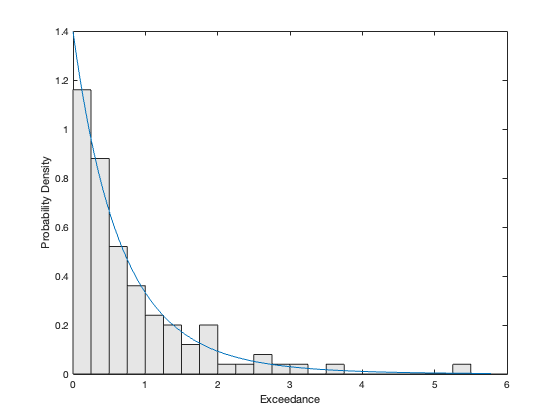
\includegraphics [width=4in]{lec4_step2_genMat4Assort_Platinum_01.eps}

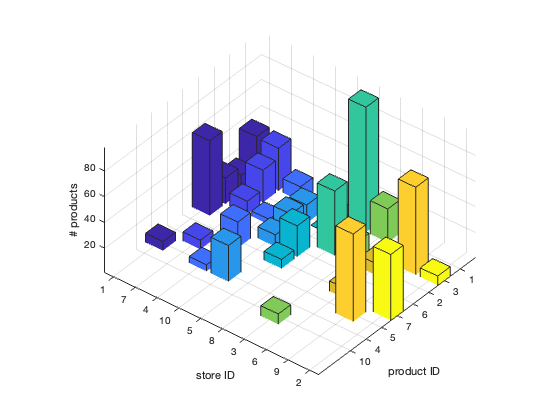
\includegraphics [width=4in]{lec4_step2_genMat4Assort_Platinum_02.eps}

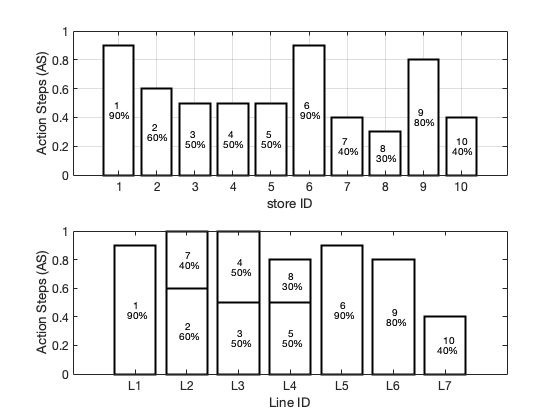
\includegraphics [width=4in]{lec4_step2_genMat4Assort_Platinum_03.eps}



\end{document}

